%=======================02-713 LaTeX template, following the 15-210 template==================
%
% You don't need to use LaTeX or this template, but you must turn your homework in as
% a typeset PDF somehow.
%
% How to use:
%    1. Update your information in section "A" below
%    2. Write your answers in section "B" below. Precede answers for all 
%       parts of a question with the command "\question{n}{desc}" where n is
%       the question number and "desc" is a short, one-line description of 
%       the problem. There is no need to restate the problem.
%    3. If a question has multiple parts, precede the answer to part x with the
%       command "\part{x}".
%    4. If a problem asks you to design an algorithm, use the commands
%       \algorithm, \correctness, \runtime to precede your discussion of the 
%       description of the algorithm, its correctness, and its running time, respectively.
%    5. You can include graphics by using the command \includegraphics{FILENAME}
%
\documentclass[11pt]{article}
\usepackage{amsmath,amssymb,amsthm}
\usepackage{graphicx}
\usepackage[margin=1in]{geometry}
\usepackage{fancyhdr}
\usepackage{listings}
\setlength{\parindent}{0pt}
\setlength{\parskip}{5pt plus 1pt}
\setlength{\headheight}{13.6pt}
\newcommand\question[2]{\vspace{.25in}\hrule\textbf{#1: #2}\vspace{.5em}\hrule\vspace{.10in}}
\renewcommand\part[1]{\vspace{.10in}\textbf{(#1)}}
\newcommand\singlelayer{\vspace{.10in}\textbf{Single-Layer Neural Networks: }}
\newcommand\multilayer{\vspace{.10in}\textbf{Multi-Layer Neural Networks: }}
\newcommand\snn{\vspace{.10in}\textbf{Shallow Neural Networks: }}
\newcommand\dnn{\vspace{.10in}\textbf{Deep Neural Networks: }}
\newcommand\al{\vspace{.10in}\textbf{Algorithm: }}
\newcommand\op{\vspace{.10in}\textbf{Output: }}


\pagestyle{fancyplain}
\lhead{\textbf{\NAME\ (\ANDREWID)}}
\chead{\textbf{Lab\HWNUM}}
\rhead{\today}
\begin{document}\raggedright
%Section A==============Change the values below to match your information==================
\newcommand\NAME{Yao Xiao}  % your name
\newcommand\ANDREWID{2019180015}     % your andrew id
\newcommand\HWNUM{1}              % the homework number
%Section B==============Put your answers to the questions below here=======================

% no need to restate the problem --- the graders know which problem is which,
% but replacing "The First Problem" with a short phrase will help you remember
% which problem this is when you read over your homeworks to study.

\question{1}{The First Problem} 

\part{a} \singlelayer \\A single-layer neural network represents the most simple form of neural network, in which there is only one layer of input nodes that send weighted inputs to a subsequent layer of receiving nodes, or in some cases, one receiving node.\\
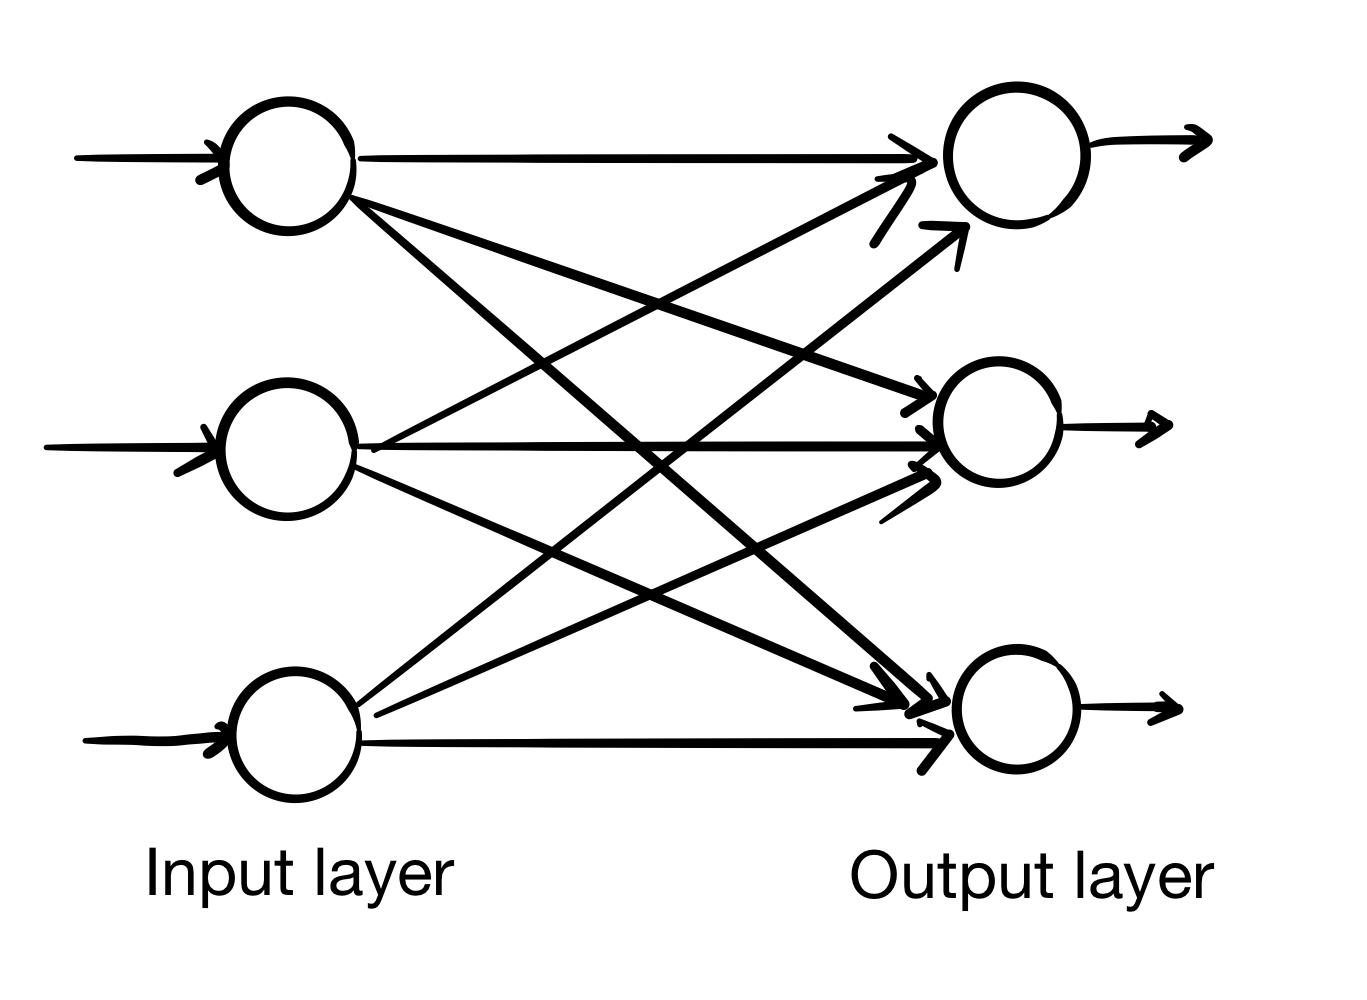
\includegraphics[scale=0.15]{sl.jpeg}

\part{b} \multilayer \\A multi-layer neural network contains more than one layer of artificial neurons or nodes. Typically, they have at least one input layer, which sends weighted inputs to a series of hidden layers, and an output layer at the end.\\
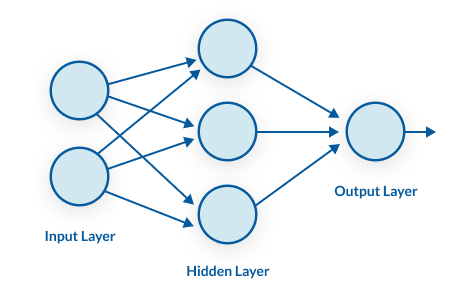
\includegraphics[scale=0.6]{ml.png}

\part{c} \snn \\A shallow neural network simply consist of one hidden layer between the input and the output.\\
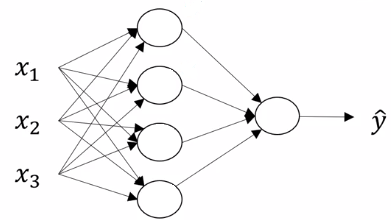
\includegraphics[scale=0.45]{snn.png}

\part{d} \dnn \\A deep neural network simply consist of more than more than equal to 2 hidden layers between the input and the output.\\
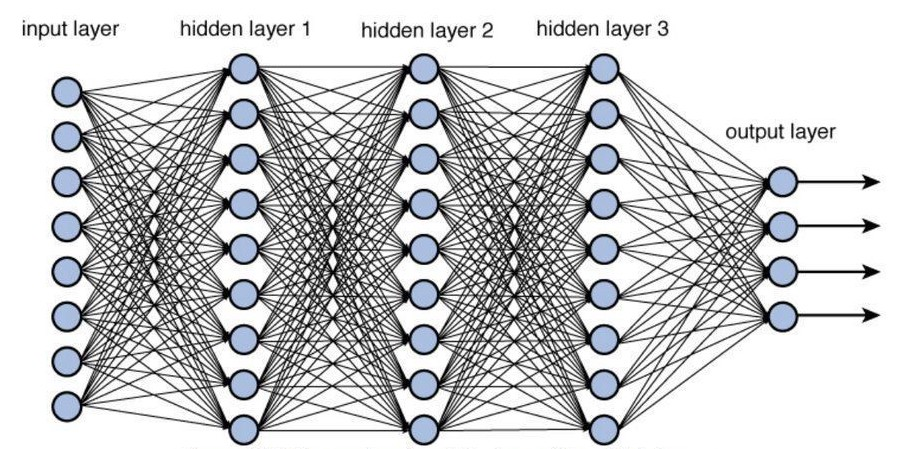
\includegraphics[scale=0.4]{dnn.jpeg}

\question{2}{The Second problem}
\part{a} \al
\begin{lstlisting}
import numpy as np

#create neurons of neural networks
class Neuron():
    def __init__(self,weights,bias):
        self.weights = weights
        self.bias = bias

#activation function
def sigmoid(x):
    return 1 / (1 + np.exp(-x))


def feedforward(w,b,inputs):
    h1_1 = np.dot(w[0:1],inputs) + b
    h1_2 = np.dot(w[1:2],inputs) + b
    t_1 = np.array([sigmoid(h1_1),sigmoid(h1_2)])
    h2_1 = np.dot(w[2:3],t_1) + b
    h2_2 = np.dot(w[3:4],t_1) + b
    return sigmoid(h2_1), sigmoid(h2_2)


#parameters w and b
weights = np.array([[3,1],[2,4],[3,2],[5,1]])
bias = 1
n = Neuron(weights,bias)

set_x = input() 
set_y = input()

inputs = np.array([int(set_x),int(set_y)])


print('The first ouput is ' + str(feedforward(n.weights,n.bias,inputs)[0]))
print('The second output is ' + str(feedforward(n.weights,n.bias,inputs)[1]))
\end{lstlisting}

\part{b} \op \\
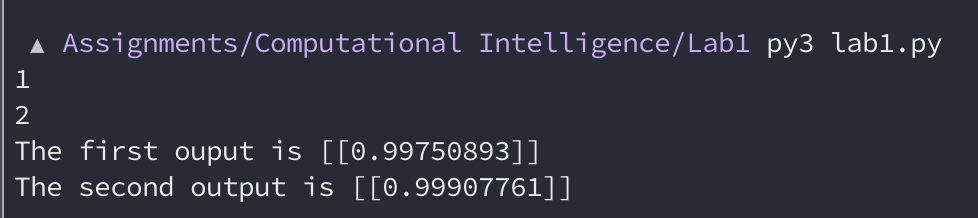
\includegraphics[]{op.png}

\end{document}
